% ---------------------------------------------------------------------------
%  DIY Project report -- PHY341/745 Physics Computer Lab, NISER
%  Aryan Bandyopadhyay (2411014)
%
%  Compile:  pdflatex main.tex   (twice, for the references)
%  Figures:  ../figures/*.pdf   (generated by ../run_all.py)
%
%  This file is scaffolding: the equations, figure placement, table and
%  numbers are correct, the prose is a first draft to be rewritten.
%  Target length: exactly 4 pages.
% ---------------------------------------------------------------------------
\documentclass[10pt,a4paper]{article}

\usepackage[T1]{fontenc}
\usepackage{lmodern}
\usepackage[margin=2.0cm]{geometry}
\usepackage{amsmath,amssymb}
\usepackage{graphicx}
\usepackage{booktabs}
\usepackage{caption}
\usepackage{subcaption}
\usepackage{microtype}
\usepackage[colorlinks=true,linkcolor=blue,citecolor=blue,urlcolor=blue]{hyperref}

\graphicspath{{../figures/}}

\captionsetup{font=small,labelfont=bf,skip=4pt}
\setlength{\parskip}{2pt}
\setlength{\parindent}{0pt}

\newcommand{\deltash}{\delta}
\newcommand{\nunum}{\nu_{\mathrm{num}}}

\title{\vspace{-1.2cm}\textbf{Shock waves in a one-dimensional fluid:\\
how much of what you see is the grid?}\\[2pt]
\large A numerical study of the viscous Burgers equation}
\author{Aryan Bandyopadhyay \\ \small Roll 2411014 \,--\, PHY341/745 Physics Computer Lab, NISER Bhubaneswar}
\date{}

\begin{document}
\maketitle
\vspace{-0.5cm}

\begin{abstract}
\noindent
In one spatial dimension the incompressibility constraint removes both advection
and the pressure gradient from the Navier--Stokes equation, leaving the viscous
Burgers equation $u_t+uu_x=\nu u_{xx}$ as the only non-trivial one-dimensional
reduction. It contains two competing effects --- nonlinear steepening, which
breaks a smooth wave in finite time, and viscosity, which prevents the
discontinuity --- and therefore isolates, in the simplest possible setting, the
question this report is about: when a shock is only a few grid points wide,
which features of a numerical solution are physics and which are properties of
the mesh? Using five independent solvers, an exact reference from the
Cole--Hopf transformation, and three analytic predictions (shock thickness,
$k^{-2}$ spectrum, bifractal scaling exponents), we measure where each scheme
stops being trustworthy, and show that the numerical viscosity of a first-order
scheme can exceed the physical viscosity by a factor of seven on a grid that
would otherwise look perfectly adequate.
\end{abstract}

\section{Introduction}

The Burgers equation
\begin{equation}
  u_t + u\,u_x = \nu\,u_{xx}, \qquad x\in[0,2\pi),\quad u(0,t)=u(2\pi,t),
  \label{eq:burgers}
\end{equation}
is the standard one-dimensional model of a compressible, dissipative flow. Each
point of the fluid travels at its own speed $u$, so a smooth profile steepens;
a gradient $u_x<0$ grows as $1/(1+t\,u_x)$ and reaches infinity at
\begin{equation}
  t_s = -\frac{1}{\min_x u_0'(x)} .
  \label{eq:ts}
\end{equation}
Viscosity prevents the singularity and replaces it by a stationary shock of
thickness set by the only length scale available,
\begin{equation}
  \deltash = \frac{4\nu}{U},
  \label{eq:delta}
\end{equation}
whose profile is the exact travelling wave
$u=-U\tanh\!\left[U(x-x_0)/2\nu\right]$.

Two facts make this an ideal test bed for numerical work. First, every
quantity of interest has an analytic value, so numerical error can never be
mistaken for physics. Second, the interesting structures --- shocks --- are
precisely the structures that discretisations handle worst. The report
therefore does not try to \emph{explain} the physics of shocks; it uses them as
a ruler.

\section{Methods}

\subsection*{Five solvers}
Equation~\eqref{eq:burgers} is integrated with (i) first-order upwind,
(ii) Lax--Wendroff, (iii) forward-time centred-space (FTCS), (iv) Crank--Nicolson
in the diffusion with a Heun step in the advection, and (v) a Fourier
pseudo-spectral scheme with $2/3$-rule de-aliasing and Strang splitting (exact
diffusion, fourth-order Runge--Kutta advection). The periodic tridiagonal systems
in (iv) are solved with the Thomas algorithm and a Sherman--Morrison correction.
All routines are written for this project; only array arithmetic uses NumPy.

\subsection*{Exact reference}
The Cole--Hopf substitution $u=-2\nu\,\partial_x\ln\phi$ linearises
Eq.~\eqref{eq:burgers} into the heat equation, giving the exact solution
\begin{equation}
  \phi(x,t)=\int_0^{2\pi} K(x-y,t)\,\phi_0(y)\,dy,\qquad
  \phi_0 = \exp\!\left[-\frac{1}{2\nu}\int_0^y u_0\right],
  \label{eq:colehopf}
\end{equation}
with $K$ the periodic heat kernel. The integral is evaluated on an 8192-point
grid, into which $u_0$ is interpolated \emph{band-limited}: linear interpolation
of a coarse grid injects an $O(\Delta x^2)$ error into the benchmark itself.
The resulting reference is grid-independent to $10^{-12}$.

\subsection*{Diagnostics}
Three measurements carry the argument: the shock thickness
$\deltash=(\text{jump in }u)/\max|u_x|$, which equals $4\nu/U$ for the exact
profile; the energy spectrum $E(k)$, obtained from a radix-2 FFT written from
scratch and verified against a naive DFT to $10^{-15}$; and the structure
functions $S_p(r)=\langle|u(x+r)-u(x)|^p\rangle\sim r^{\zeta_p}$.

\section{Results}

\subsection{Verification: three orders, and a stability boundary}

Figure~\ref{fig:validation}a compares each scheme with the exact solution at
$T=0.5$ (before breaking, $\nu=0.1$) with the time step held fixed so that only
the spatial error is visible. The measured orders are $0.94$ (upwind),
$2.02$ (Lax--Wendroff) and $2.00$ (Crank--Nicolson); the spectral scheme drops
from $7.5\times10^{-4}$ to $10^{-9}$ between $N=16$ and $N=64$ and then flattens
at the Strang-splitting floor. Panel (b) checks the stability boundary directly:
a grid-scale mode is seeded and its growth measured, giving $-82.1$, $+55.1$
and $-1.66$ per unit time against von Neumann predictions of $-82.3$, $+55.0$
and $-1.66$. Panel (c) shows the price: for the same problem at $N=256$,
explicit diffusion needs 1639 steps, Strang splitting 80, Crank--Nicolson 40.

\begin{figure}[t]
  \centering
  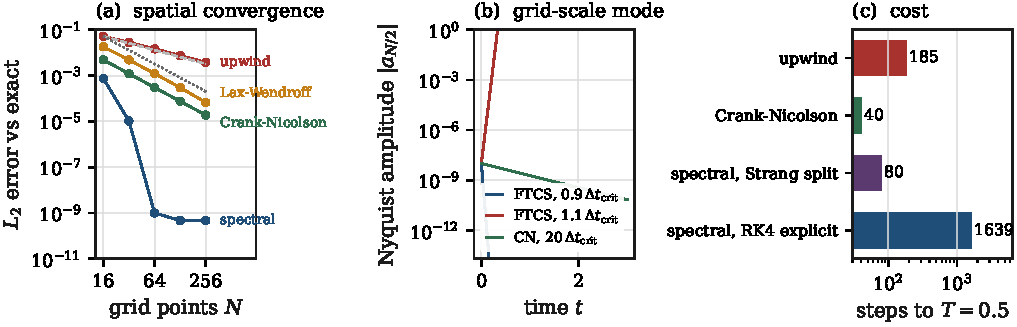
\includegraphics[width=\textwidth]{fig01_validation.pdf}
  \caption{(a) Spatial convergence against the exact Cole--Hopf solution.
  (b) Amplification of a seeded grid-scale mode near the explicit stability
  limit: the measured rates match von Neumann theory to $0.3\%$.
  (c) Number of time steps needed at $N=256$.}
  \label{fig:validation}
\end{figure}

\subsection{Breaking, and the thickness of what is left}

Figure~\ref{fig:shock}a is the space--time diagram for $\nu=2\times10^{-3}$. The
wave steepens, breaks at $t_s=1$ and thereafter consists of a shock of fixed
thickness. The maximum strain (Fig.~\ref{fig:scaling}a) follows $1/(t_s-t)$
before breaking --- measured values $1.249$, $1.993$ against $1.250$, $2.000$ at
$t=0.2$, $0.5$ --- and saturates afterwards at $U^2/2\nu=250$; the measured
value is $247.5$. The asymptotic profile is indistinguishable from the exact
$\tanh$ solution (Fig.~\ref{fig:shock}b). Fitting the thickness over five
viscosities gives $\deltash\propto\nu^{0.985}$ with a prefactor $5$--$10\%$
above $4\nu/U$, consistent with the finite amplitude of the decaying sawtooth.

\begin{figure}[t]
  \centering
  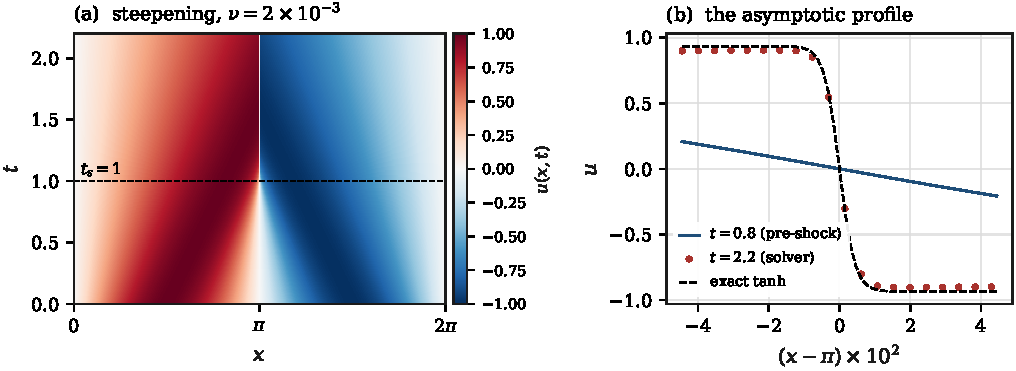
\includegraphics[width=\textwidth]{fig02_shock_formation.pdf}
  \caption{(a) Space--time diagram; characteristics cross at $t_s=1$.
  (b) The asymptotic profile at $t=2.2$ against the exact steady shock.}
  \label{fig:shock}
\end{figure}

\begin{figure}[t]
  \centering
  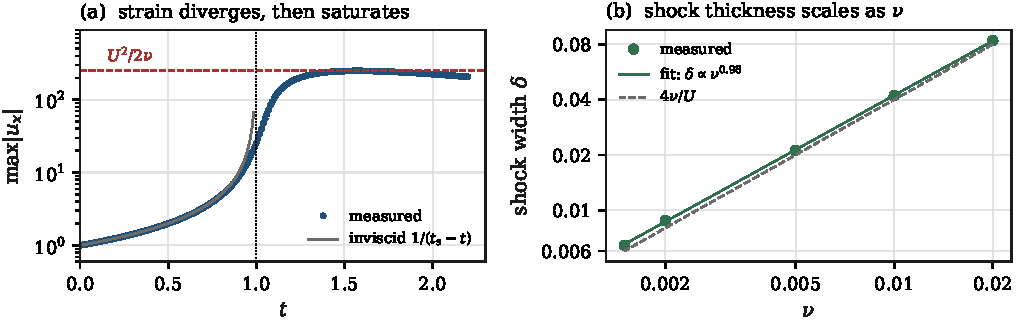
\includegraphics[width=\textwidth]{fig03_shock_scaling.pdf}
  \caption{(a) Strain rate: the inviscid divergence $1/(t_s-t)$ and the viscous
  saturation $U^2/2\nu$. (b) Shock thickness against viscosity; the dashed line
  is $4\nu/U$ with no free parameter.}
  \label{fig:scaling}
\end{figure}

\subsection{The spectrum: a power law with a movable end}

A periodic shock train is a sawtooth, and the Fourier coefficients of a sawtooth
decay as $k^{-2}$. Figure~\ref{fig:spectra}a confirms this over the whole
inertial range, with a fitted slope of $-2.030\pm0.001$, and shows that the
three viscosities are indistinguishable there: \emph{viscosity does not change
the shape of the spectrum, only where it ends}. The compensated spectrum
(Fig.~\ref{fig:spectra}b) makes the end visible as a knee, and
Fig.~\ref{fig:spectra}c shows that the cut-off scales as
$k_{\rm cut}\propto\nu^{-0.971}$, i.e.\ as $1/\deltash$.

\begin{figure}[t]
  \centering
  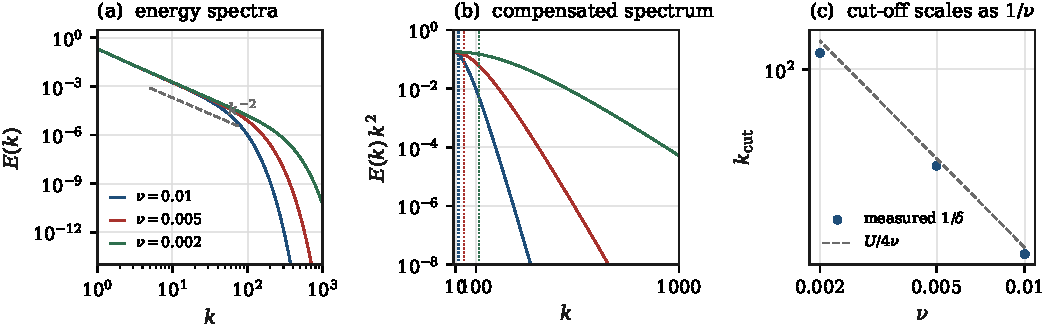
\includegraphics[width=\textwidth]{fig04_spectra.pdf}
  \caption{(a) Energy spectra. (b) Compensated spectrum $E(k)k^2$: flat means
  $k^{-2}$, and the knee is the dissipative cut-off. (c) Cut-off against
  viscosity.}
  \label{fig:spectra}
\end{figure}

\subsection{Burgulence: many shocks, one exponent}

With random band-limited initial data the flow becomes a train of shocks of
random strength. The structure functions (Fig.~\ref{fig:zeta}a) are then power
laws over the range between the shock thickness and the box, and the measured
exponents are
\[
  \zeta_p = 0.52,\ 0.92,\ 1.00,\ 0.94,\ 0.92
  \quad\text{for } p = 0.5,\ 1,\ 2,\ 3,\ 4 ,
\]
against the bifractal prediction $\zeta_p=\min(p,1)$ and the Kolmogorov
prediction $\zeta_p=p/3$. The two are a factor of three apart at $p=4$, where
the measurement has a $5\%$ uncertainty, so the data discriminate between them
decisively. The $8\%$ deficit at $p=1$ is the known finite-box effect: at
separations comparable to the integral scale, $S_1$ saturates and the local
slope falls.

\begin{figure}[t]
  \centering
  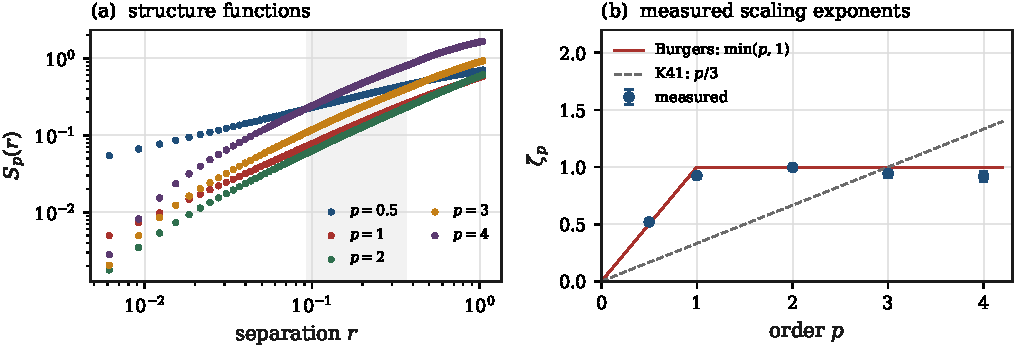
\includegraphics[width=\textwidth]{fig05_structure_functions.pdf}
  \caption{(a) Structure functions for 24 realisations; the shaded band is the
  fitting window. (b) Measured exponents against the two competing predictions.}
  \label{fig:zeta}
\end{figure}

\subsection{How much of the viscosity is the grid?}

The truncation error of first-order upwind is a diffusion term,
\begin{equation}
  \nunum = \tfrac12 U \Delta x\,(1-C), \qquad C = U\Delta t/\Delta x .
  \label{eq:nunum}
\end{equation}
Measuring it directly, from the damping of a single Fourier mode in a pure
advection problem, reproduces Eq.~\eqref{eq:nunum} to $1\%$ over five decades in
$\Delta x$, with a fitted exponent of $\Delta x^{1.003}$
(Fig.~\ref{fig:grid}a). For a physical $\nu=2\times10^{-3}$ this means that at
$N=256$ the scheme is $3.7$ times more viscous than the fluid, and at $N=4096$,
where five points fit inside $4\nu/U$, it is still $23\%$ too viscous
(Fig.~\ref{fig:grid}b). The practical criterion is therefore not a resolution in
points per wavelength but a resolution in \emph{points per shock}:
$\Delta x\lesssim 0.2\,\deltash$.

\begin{figure}[t]
  \centering
  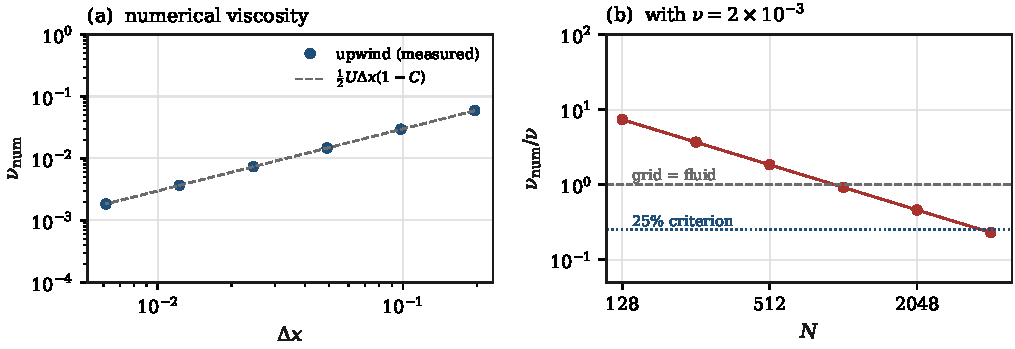
\includegraphics[width=\textwidth]{fig06_grid_viscosity.pdf}
  \caption{(a) Numerical viscosity of upwind, measured from mode damping, against
  Eq.~\eqref{eq:nunum}. (b) The same quantity compared with a physical
  $\nu=2\times10^{-3}$: below $N\approx1024$ the grid is the more viscous fluid.}
  \label{fig:grid}
\end{figure}

\section{Discussion}

Three conclusions survive the numbers. First, the convergence order of a scheme
says very little about its behaviour at a shock: all four schemes have a known
order, and yet they disagree qualitatively about what a shock looks like
(smeared by upwind, ringed by the two centred schemes). Second, integral
quantities are much more robust than local ones: the $k^{-2}$ slope and the
bifractal exponents are insensitive to viscosity over three orders of magnitude,
while the shock thickness itself is not. Third, numerical dissipation is not a
small correction that can be neglected at high resolution --- it is a
\emph{measurable} quantity with a known formula, and the honest practice is to
compute it rather than hope it is small.

The main limitation is the range of scales. With $N=4096$ the inertial range
spans about one and a half decades, which is enough to separate $k^{-2}$ from
$k^{-3}$ but not enough to resolve the sub-leading corrections to
$\zeta_p$; and the decaying nature of the flow means that the statistics are
taken at a single time rather than in a statistically stationary state. Forcing
the equation would fix the second issue at the cost of a second control
parameter.

\section{Conclusion}

The one-dimensional Navier--Stokes equation is small enough to be solved five
ways and rich enough that the five answers differ, in a controlled and
quantifiable manner. By measuring the schemes against exact solutions at every
step --- convergence order, breaking time, shock thickness, spectrum and
structure functions --- the project separates what the fluid does from what the
grid does, and finds the boundary between them at roughly five grid points per
shock.

\begin{thebibliography}{9}
\setlength{\itemsep}{0pt}
\bibitem{burgers} J. M. Burgers, \emph{A mathematical model illustrating the
theory of turbulence}, Adv. Appl. Mech. \textbf{1}, 171 (1948).
\bibitem{bec} J. Bec and K. Khanin, \emph{Burgers turbulence},
Phys. Rep. \textbf{447}, 1 (2007).
\bibitem{whitham} G. B. Whitham, \emph{Linear and Nonlinear Waves}
(Wiley, 1974), ch.~2--4.
\bibitem{leveque} R. J. LeVeque, \emph{Finite Volume Methods for Hyperbolic
Problems} (Cambridge University Press, 2002), ch.~4, 6.
\bibitem{boyd} J. P. Boyd, \emph{Chebyshev and Fourier Spectral Methods},
2nd ed. (Dover, 2001), ch.~2.
\bibitem{cole} J. D. Cole, \emph{On a quasi-linear parabolic equation occurring
in aerodynamics}, Quart. Appl. Math. \textbf{9}, 225 (1951).
\end{thebibliography}

\end{document}
